% Supplementary I — Journal cross-section visual annex
% Topic ↔ category / measurement relational visualisations.

\documentclass[11pt,a4paper]{article}
% Shared preamble for all supplementary chapter documents.
% Used by each supplementary/conference/suppl_*.tex and
% supplementary/journal/suppl_*.tex via % Shared preamble for all supplementary chapter documents.
% Used by each supplementary/conference/suppl_*.tex and
% supplementary/journal/suppl_*.tex via % Shared preamble for all supplementary chapter documents.
% Used by each supplementary/conference/suppl_*.tex and
% supplementary/journal/suppl_*.tex via \input{../preamble.tex}.

\usepackage[utf8]{inputenc}
\usepackage[T1]{fontenc}
\usepackage[a4paper,margin=2.2cm]{geometry}
\usepackage{amsmath,amssymb,amsfonts,amsthm}
\usepackage{mathtools}
\usepackage{graphicx}
\usepackage{booktabs}
\usepackage{array}
\usepackage{multirow}
\usepackage{longtable}
\usepackage{algorithm}
\usepackage{algpseudocode}
\usepackage{xcolor}
\usepackage{url}
\usepackage{cite}
\usepackage[hidelinks]{hyperref}

\graphicspath{{../../figures/}}

\renewcommand{\thesection}{\Alph{section}.\arabic{section}}
\renewcommand{\thesubsection}{\thesection.\arabic{subsection}}

\theoremstyle{plain}
\newtheorem{theorem}{Theorem}[section]
\newtheorem{lemma}[theorem]{Lemma}
\newtheorem{proposition}[theorem]{Proposition}
\theoremstyle{definition}
\newtheorem{definition}[theorem]{Definition}
\theoremstyle{remark}
\newtheorem{remark}[theorem]{Remark}

\setcounter{secnumdepth}{3}
\setcounter{tocdepth}{2}

\newcommand{\R}{\mathbb{R}}
\newcommand{\E}{\mathbb{E}}
\newcommand{\KL}[2]{\mathrm{KL}\!\left(#1 \,\middle\|\, #2\right)}
\newcommand{\ari}{\mathrm{ARI}}
\newcommand{\nmi}{\mathrm{NMI}}
\newcommand{\softmax}{\mathrm{softmax}}
.

\usepackage[utf8]{inputenc}
\usepackage[T1]{fontenc}
\usepackage[a4paper,margin=2.2cm]{geometry}
\usepackage{amsmath,amssymb,amsfonts,amsthm}
\usepackage{mathtools}
\usepackage{graphicx}
\usepackage{booktabs}
\usepackage{array}
\usepackage{multirow}
\usepackage{longtable}
\usepackage{algorithm}
\usepackage{algpseudocode}
\usepackage{xcolor}
\usepackage{url}
\usepackage{cite}
\usepackage[hidelinks]{hyperref}

\graphicspath{{../../figures/}}

\renewcommand{\thesection}{\Alph{section}.\arabic{section}}
\renewcommand{\thesubsection}{\thesection.\arabic{subsection}}

\theoremstyle{plain}
\newtheorem{theorem}{Theorem}[section]
\newtheorem{lemma}[theorem]{Lemma}
\newtheorem{proposition}[theorem]{Proposition}
\theoremstyle{definition}
\newtheorem{definition}[theorem]{Definition}
\theoremstyle{remark}
\newtheorem{remark}[theorem]{Remark}

\setcounter{secnumdepth}{3}
\setcounter{tocdepth}{2}

\newcommand{\R}{\mathbb{R}}
\newcommand{\E}{\mathbb{E}}
\newcommand{\KL}[2]{\mathrm{KL}\!\left(#1 \,\middle\|\, #2\right)}
\newcommand{\ari}{\mathrm{ARI}}
\newcommand{\nmi}{\mathrm{NMI}}
\newcommand{\softmax}{\mathrm{softmax}}
.

\usepackage[utf8]{inputenc}
\usepackage[T1]{fontenc}
\usepackage[a4paper,margin=2.2cm]{geometry}
\usepackage{amsmath,amssymb,amsfonts,amsthm}
\usepackage{mathtools}
\usepackage{graphicx}
\usepackage{booktabs}
\usepackage{array}
\usepackage{multirow}
\usepackage{longtable}
\usepackage{algorithm}
\usepackage{algpseudocode}
\usepackage{xcolor}
\usepackage{url}
\usepackage{cite}
\usepackage[hidelinks]{hyperref}

\graphicspath{{../../figures/}}

\renewcommand{\thesection}{\Alph{section}.\arabic{section}}
\renewcommand{\thesubsection}{\thesection.\arabic{subsection}}

\theoremstyle{plain}
\newtheorem{theorem}{Theorem}[section]
\newtheorem{lemma}[theorem]{Lemma}
\newtheorem{proposition}[theorem]{Proposition}
\theoremstyle{definition}
\newtheorem{definition}[theorem]{Definition}
\theoremstyle{remark}
\newtheorem{remark}[theorem]{Remark}

\setcounter{secnumdepth}{3}
\setcounter{tocdepth}{2}

\newcommand{\R}{\mathbb{R}}
\newcommand{\E}{\mathbb{E}}
\newcommand{\KL}[2]{\mathrm{KL}\!\left(#1 \,\middle\|\, #2\right)}
\newcommand{\ari}{\mathrm{ARI}}
\newcommand{\nmi}{\mathrm{NMI}}
\newcommand{\softmax}{\mathrm{softmax}}


\title{Journal Supplementary I --- Relating topics to labels and
covariates: a visual annex\\
{\large Companion to: \emph{Beyond Accuracy} (cross-section relational
visualisations)}}
\author{Felipe Santib\'a\~nez-Leal}
\date{2026}

\begin{document}
\maketitle

\section{Scope and motivation}

The journal main paper and its earlier supplements (A--H) defend the
twelve-axis evaluation framework F-1..F-12 with figures that are
either \emph{per-axis scalars} (paired ARI, coherence, seed
stability, etc.) or \emph{per-topic intrinsic} (basis spectra,
pairwise distances). What is left under-visualised is the
\textbf{relational} question that motivates topic modelling in the
first place: \emph{do the topics actually relate to the labels and
covariates we already have?} This supplement fills that gap with six
figures, each chosen for a distinct cognitive question, with
references to the underlying visualisation tradition.

\section{F-7 viewed relationally: topic × class soft heatmap}

\begin{figure}[h]
\centering
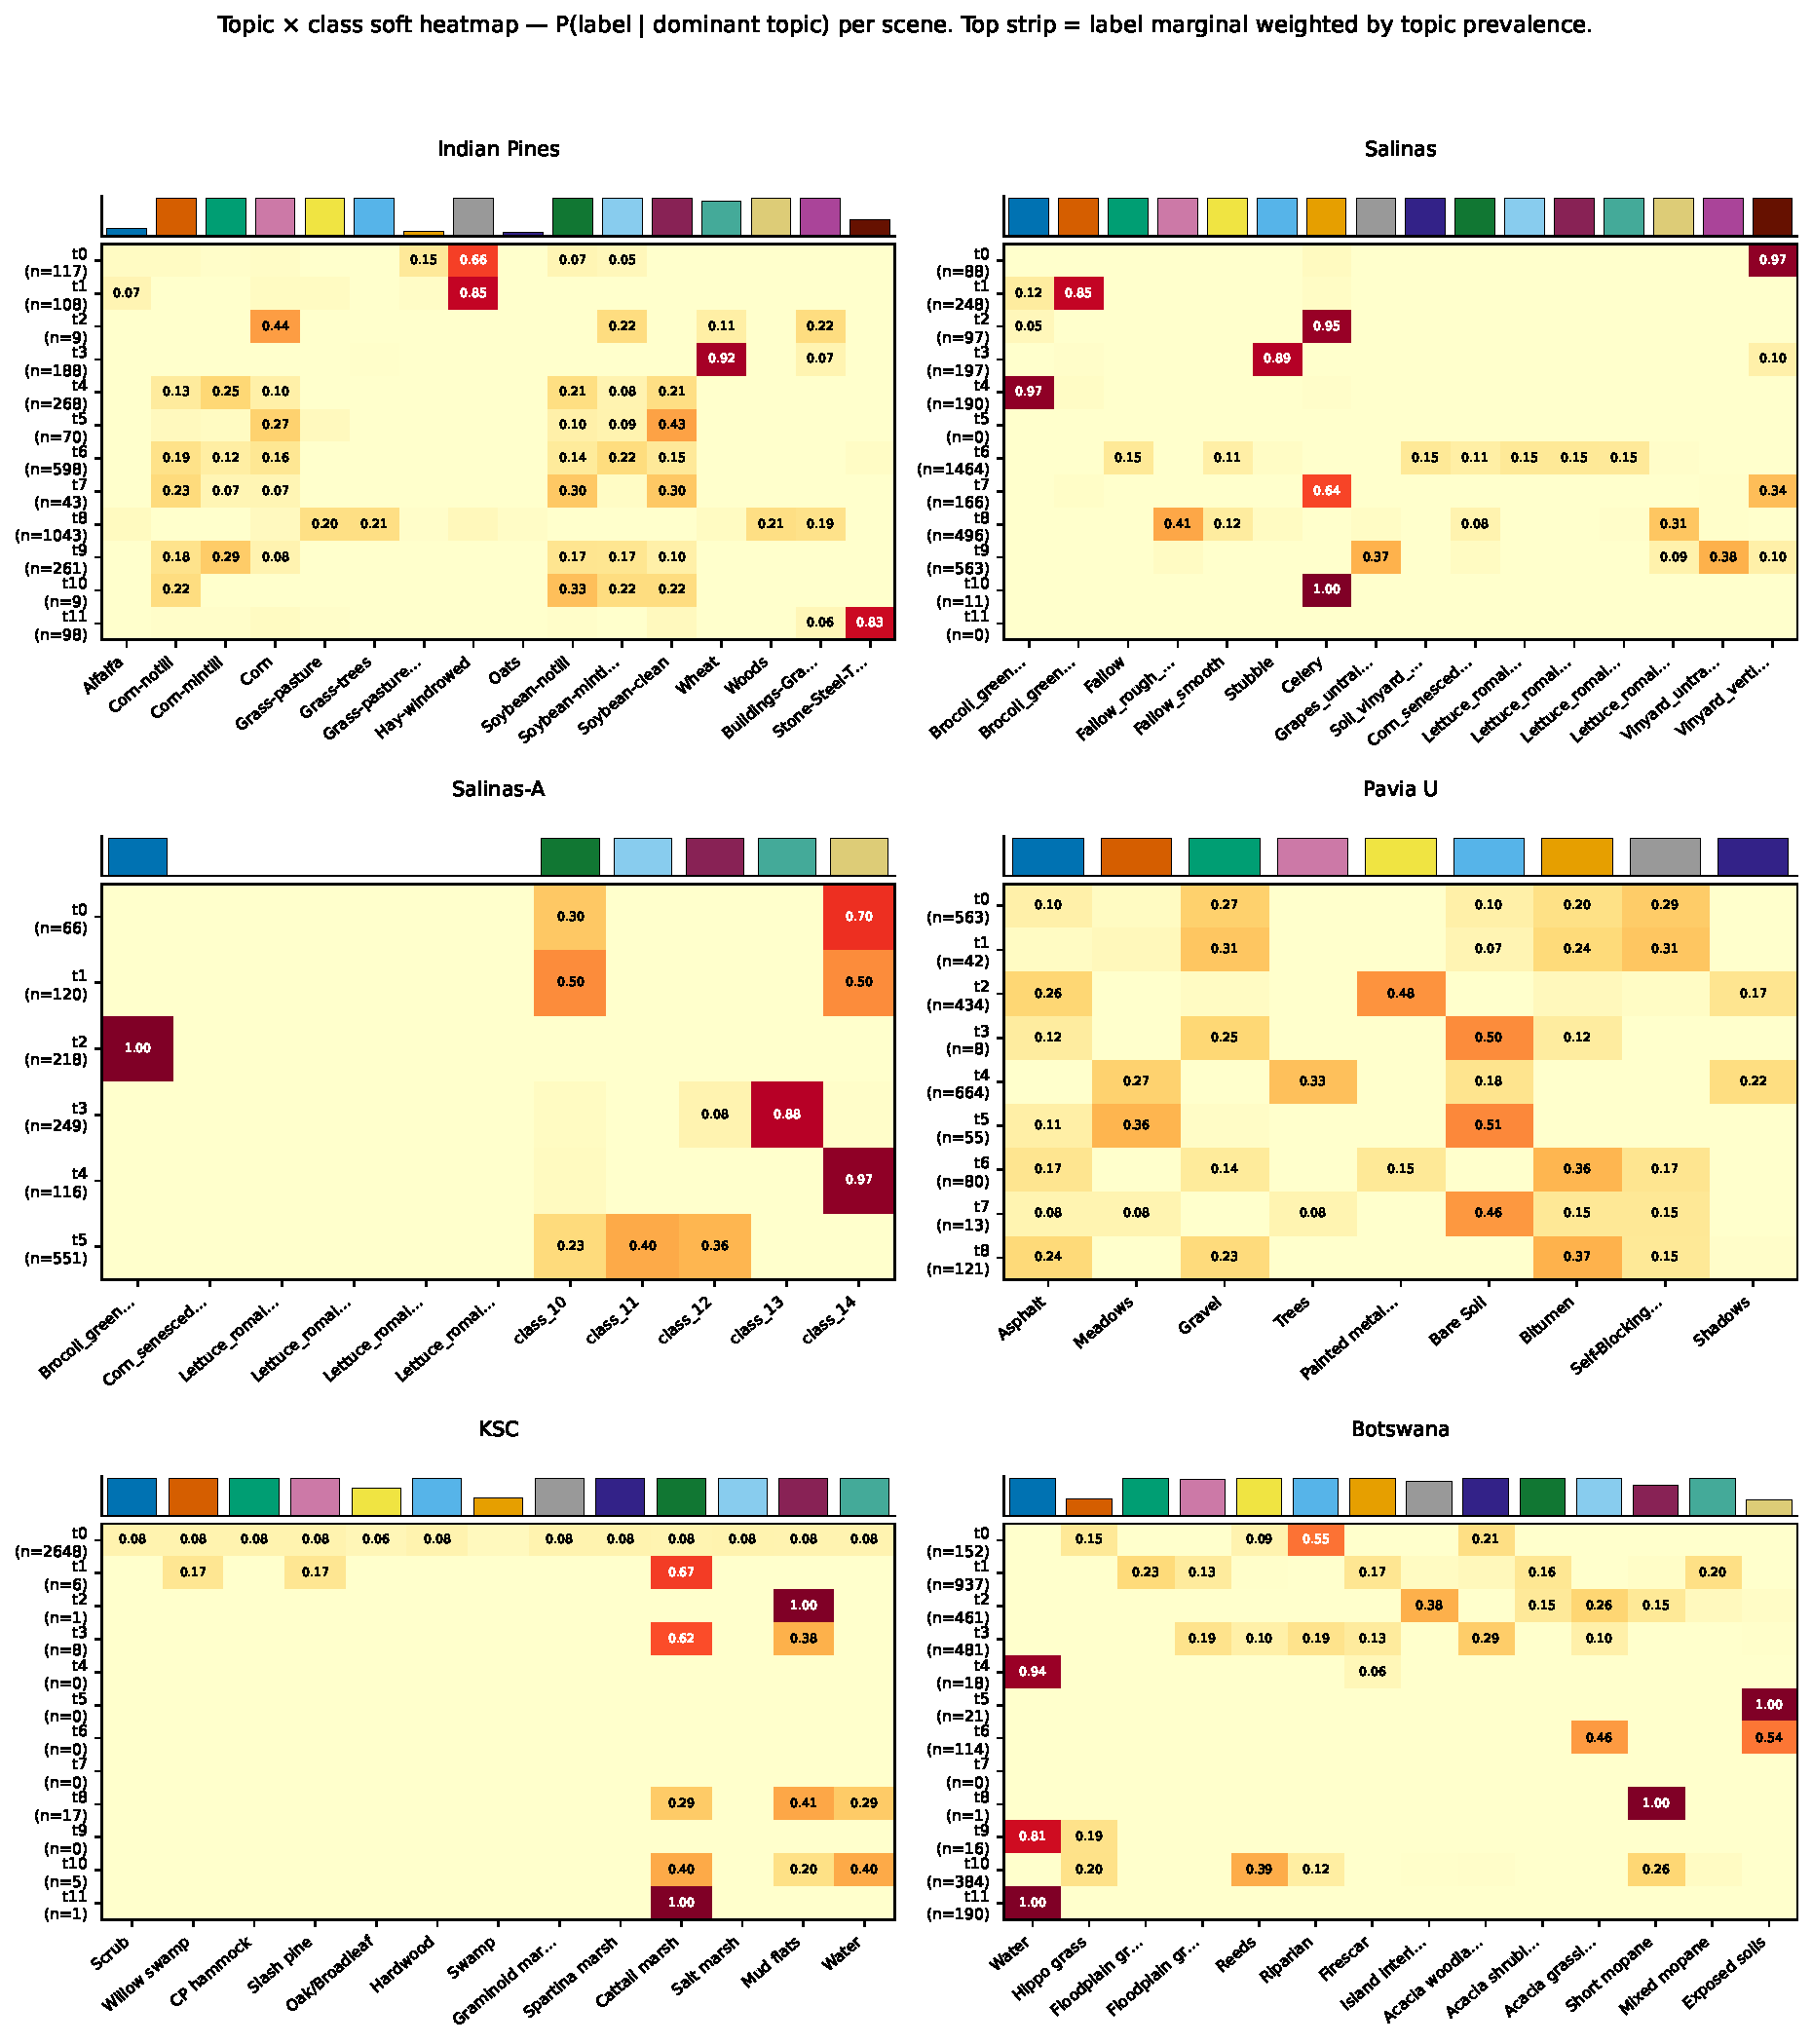
\includegraphics[width=\textwidth]{topic-class-heatmap.pdf}
\caption{Topic × class soft heatmap per labelled scene. Rows =
canonical topics (with document count); columns = ground-truth
labels; cell intensity = $P(\ell \mid t)$, the conditional label
distribution given dominant topic. Top strip = label marginal weighted
by topic prevalence. Truncated class names appear on the x-axis.}
\label{fig:tc-heatmap}
\end{figure}

This is the probabilistic generalisation of the confusion matrix.
Each cell exposes \emph{conditional label support}: a class-pure
topic has one tall cell, a mixed topic spreads across columns. The
top strip lets the reader gauge whether topic-weighted marginals
match the unconditional class prior. Following the mosaic-display
tradition of Friendly~\cite{friendly1994mosaic} and the
single-cell-LDA precedent of TITAN's \texttt{HeatmapTopic}.

\section{F-7 again: per-topic class-distribution bars}

\begin{figure}[h]
\centering
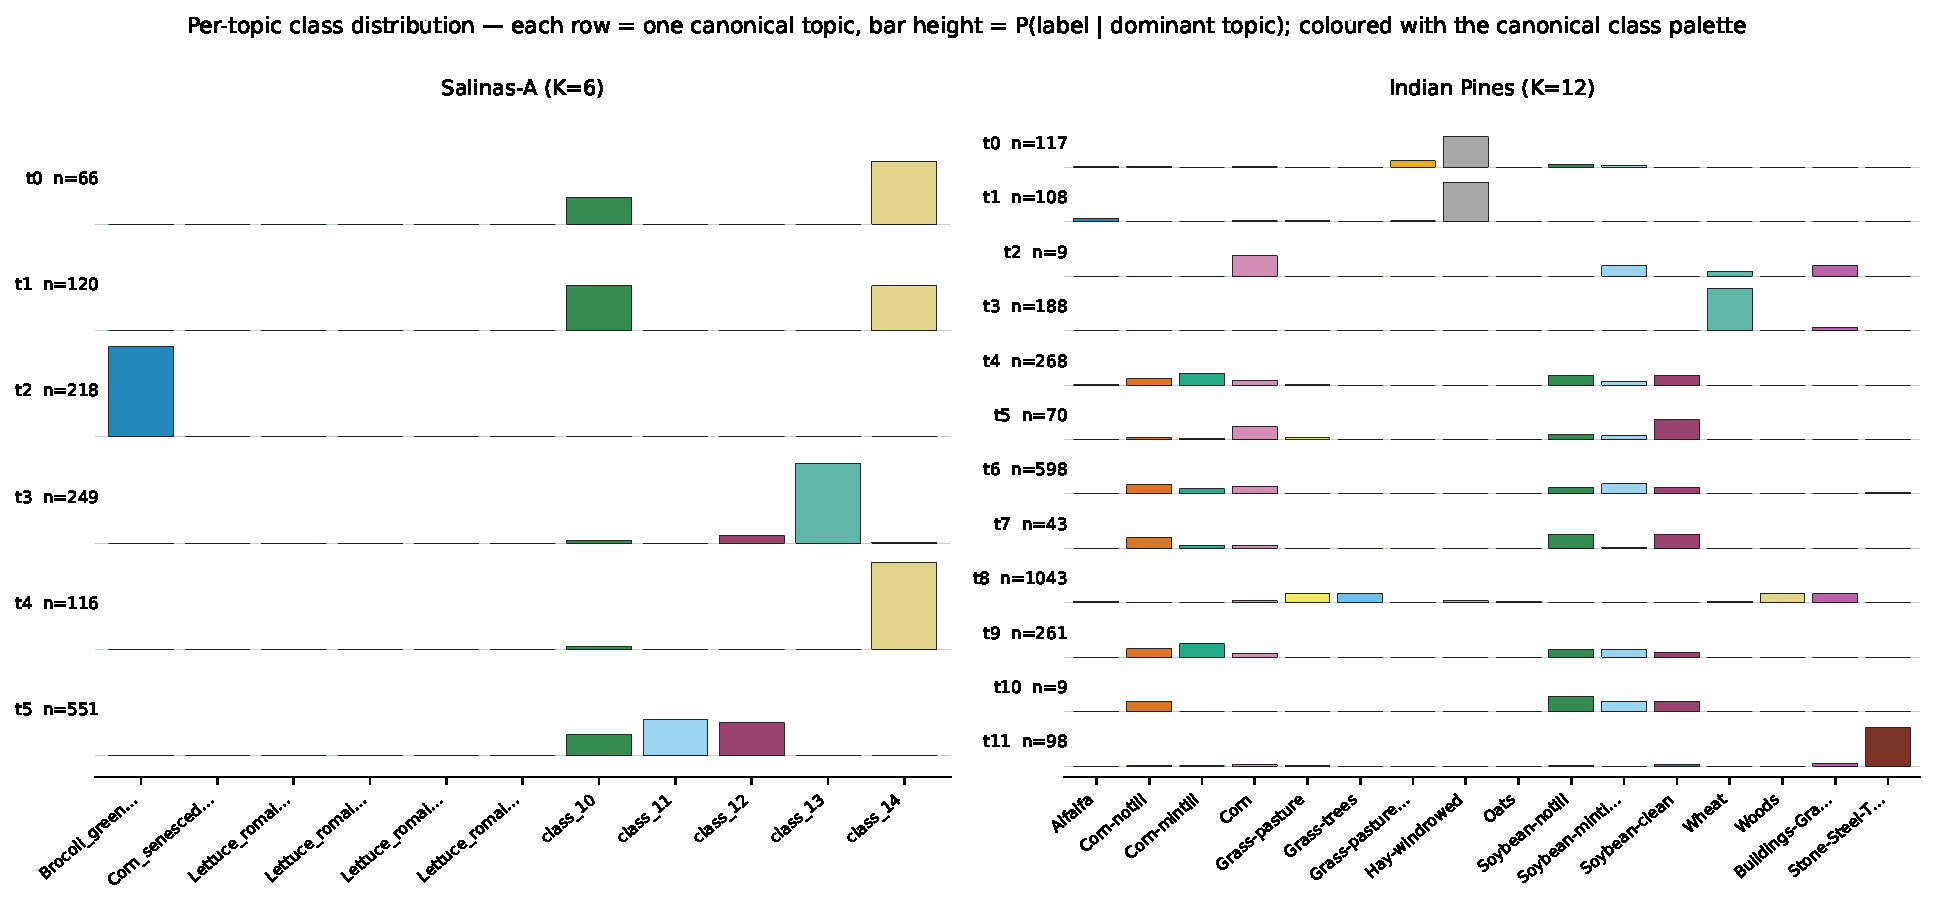
\includegraphics[width=\textwidth]{per-topic-class-bars.pdf}
\caption{Per-topic class distribution. Each row inside a panel is
one canonical topic; bar height $=P(\ell \mid t)$, coloured with the
canonical class palette so the same class is visually identifiable
across topics. A topic that resolves one or two classes shows as a
single tall bar; a topic that mixes classes shows as a spread. The
categorical analogue of the \texttt{ggridges} joy-plot
pattern~\cite{wilke2017ggridges,hintze1998violin}.}
\label{fig:tc-bars}
\end{figure}

The bars and the heatmap are duals; the heatmap optimises for
finding outlier cells, the bars optimise for reading the within-topic
distribution shape. Both ship.

\section{Topic → class Sankey / alluvial flow}

\begin{figure}[h]
\centering
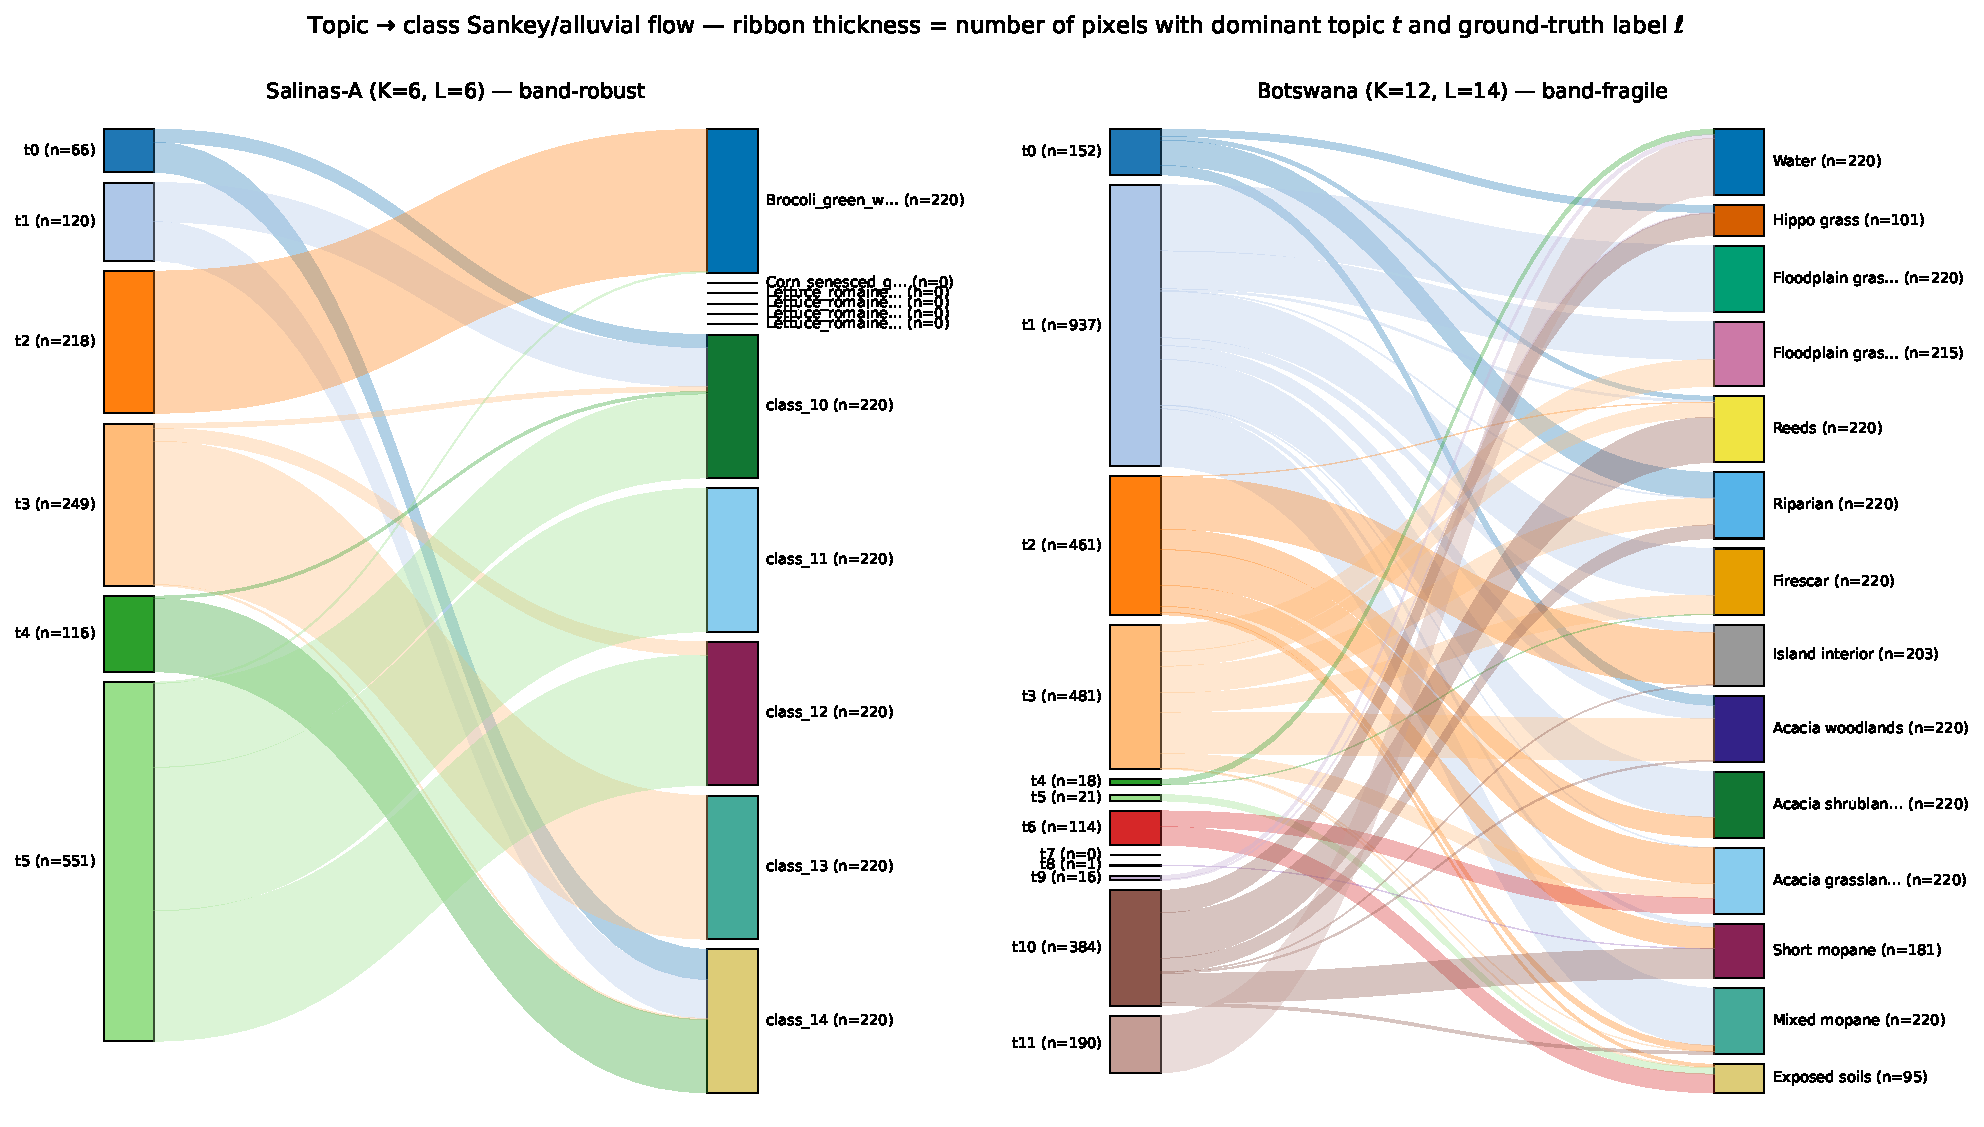
\includegraphics[width=\textwidth]{topic-class-sankey.pdf}
\caption{Topic → class Sankey/alluvial flow on Salinas-A (left) and
Botswana (right). Left axis nodes = topics; right axis nodes =
classes; ribbon width = pixel count. Salinas-A (K=6, L=6,
band-robust) shows clean alignment with thin cross-flow. Botswana
(K=12, L=14, band-fragile) shows the diffuse coupling that the
F-5 paired ARI ${\approx}\,0.01$ predicts.}
\label{fig:tc-sankey}
\end{figure}

References: Sankey diagram tradition; Data-to-Viz Sankey-vs-alluvial
distinction~\cite{datatovizSankey}; modern \texttt{d3-sankey} and
\texttt{ggsankeyfier} implementations.

\section{$\theta$-PCA scatter coloured by topic / by label}

\begin{figure}[h]
\centering
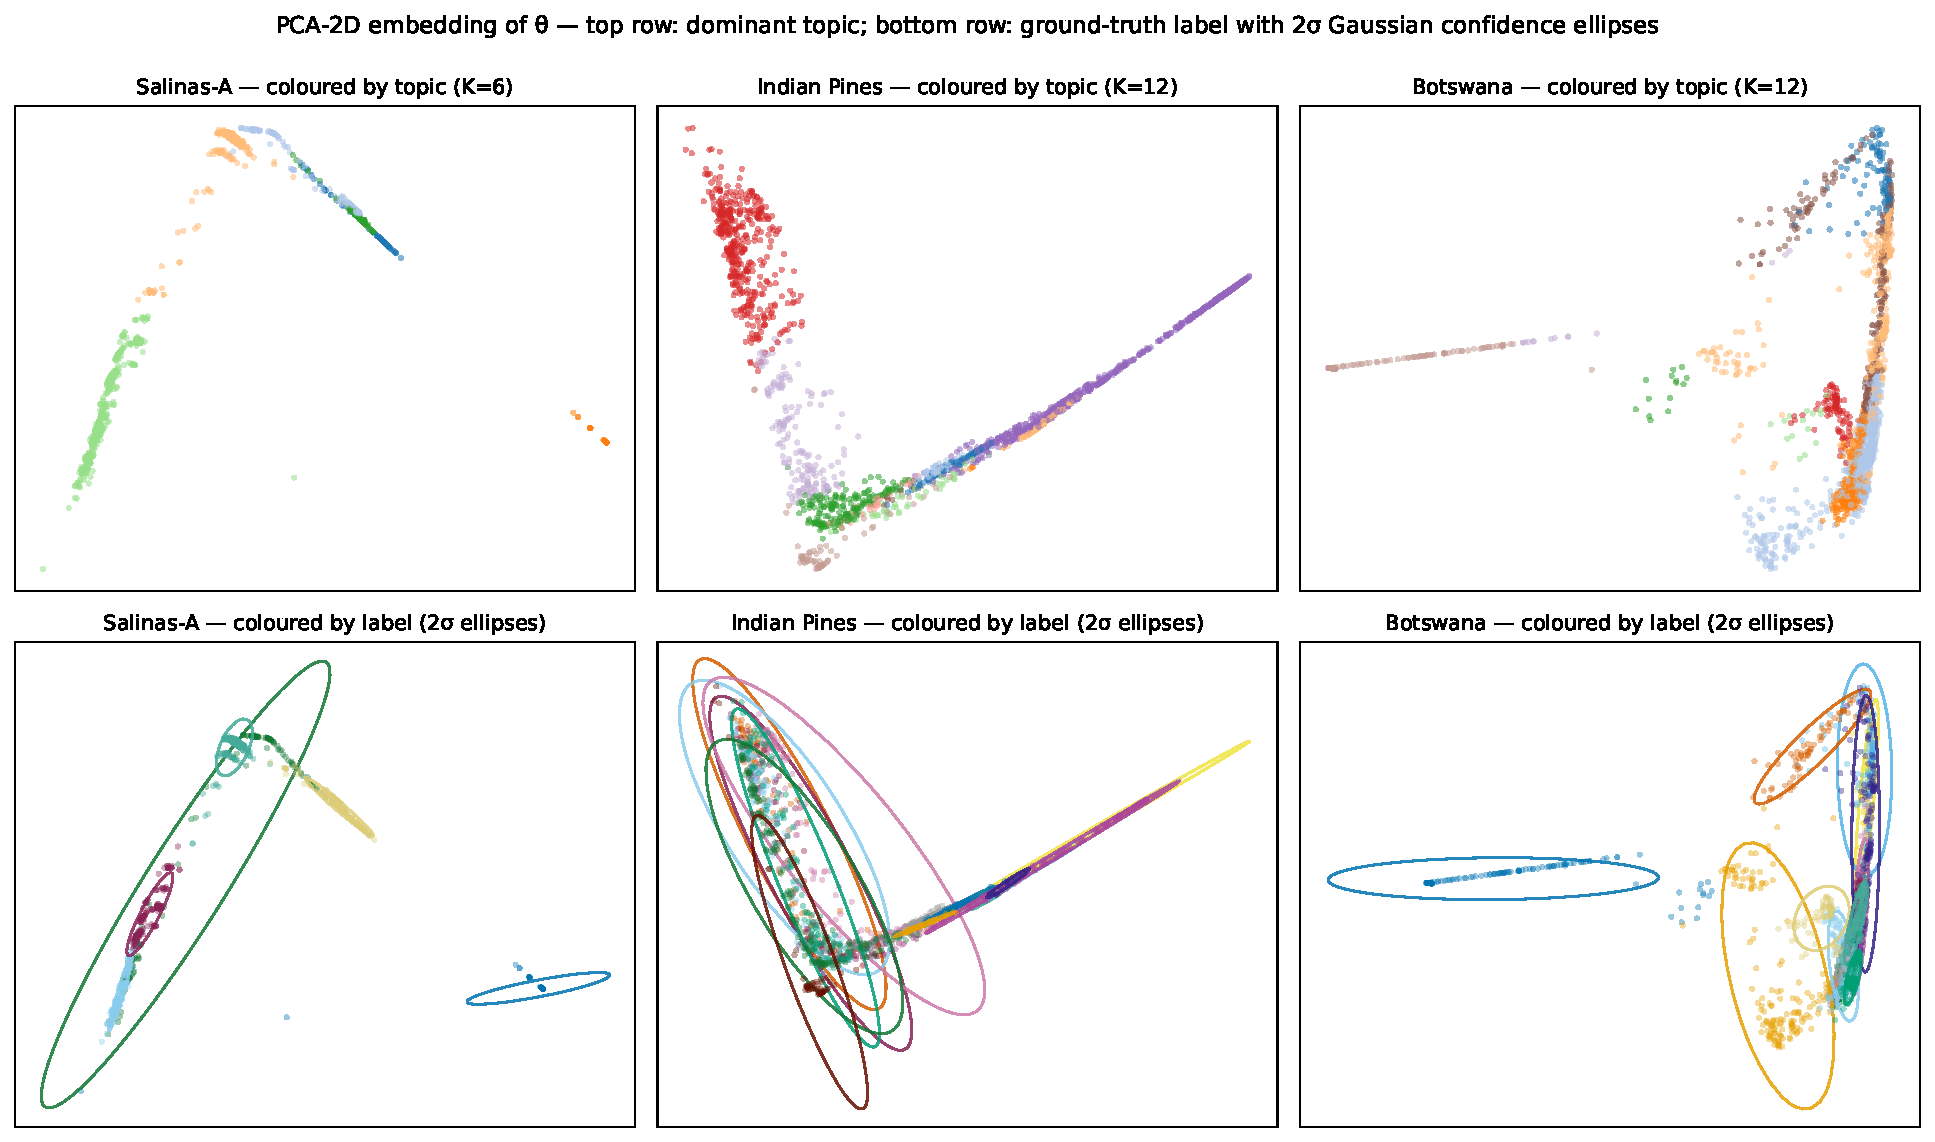
\includegraphics[width=\textwidth]{theta-embedding-scatter.pdf}
\caption{PCA-2D embedding of the per-document topic posterior
$\theta_d$ on three scenes: top row coloured by dominant topic,
bottom row coloured by ground-truth label with 2-$\sigma$ Gaussian
confidence ellipses per class. Salinas-A (band-robust): topic and
label clusters align tightly. Indian Pines (partial): topic clusters
visible but ellipses overlap. Botswana (band-fragile): topic
clusters are visible but ground-truth-label ellipses span the
whole embedding, exposing the topic--label decoupling.}
\label{fig:theta-scatter}
\end{figure}

Two-row design follows the \texttt{corner.py} scatterplot-matrix
convention of Foreman-Mackey~\cite{foremanmackey2016corner};
$2\sigma$ ellipses computed via the standard
matplotlib gallery
recipe~\cite{matplotlibConfidenceEllipse}.

\section{Per-topic confidence ridge}

\begin{figure}[h]
\centering
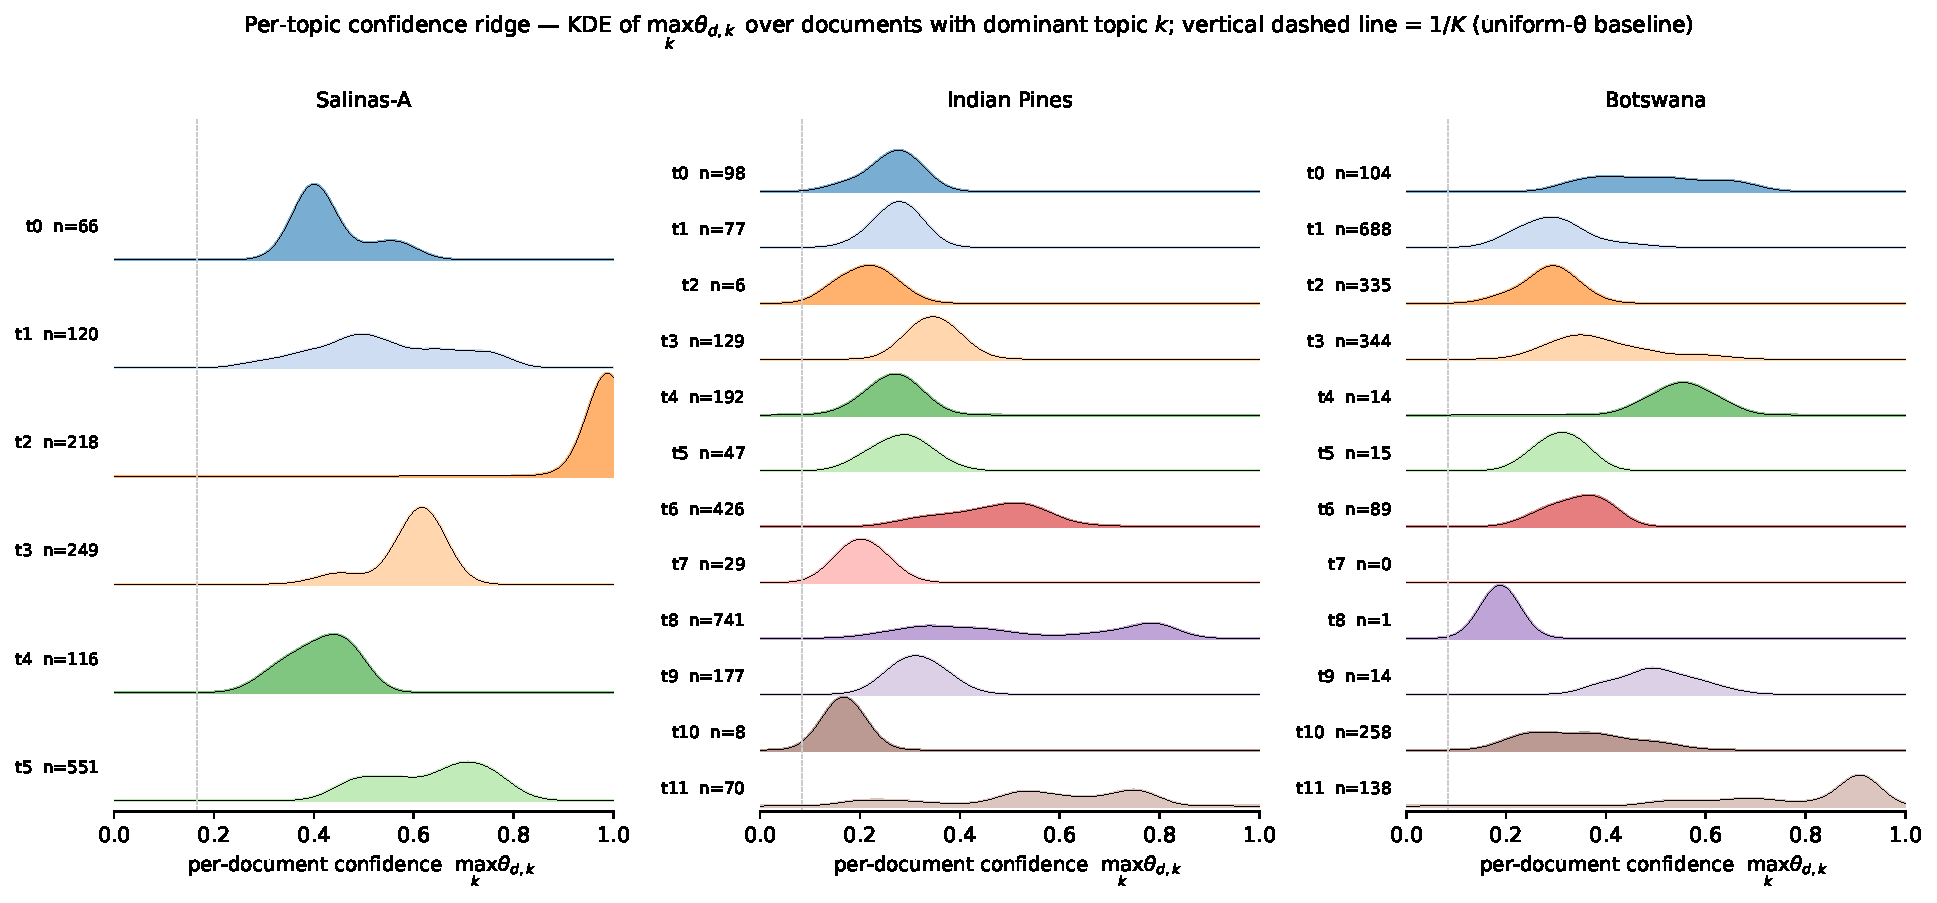
\includegraphics[width=\textwidth]{confidence-ridge.pdf}
\caption{Per-topic KDE of the per-document confidence
$\max_k \theta_{d,k}$ over documents with dominant topic $k$. Each
topic gets one ridge curve on a shared $x$-axis $[0, 1]$; vertical
dashed line at $1/K$ = uniform-$\theta$ baseline. Right-shifted
curves = sharp topics; left-shifted = diffuse / collapsed topics.}
\label{fig:conf-ridge}
\end{figure}

The ridge plot is the appropriate idiom for ``one continuous
distribution per category''. We follow Wilke's \texttt{ggridges}
naming~\cite{wilke2017ggridges}; the precursor violin-plot family
is Hintze and Nelson~\cite{hintze1998violin}.

\section{HIDSAG: topic × covariate tag}

\begin{figure}[h]
\centering
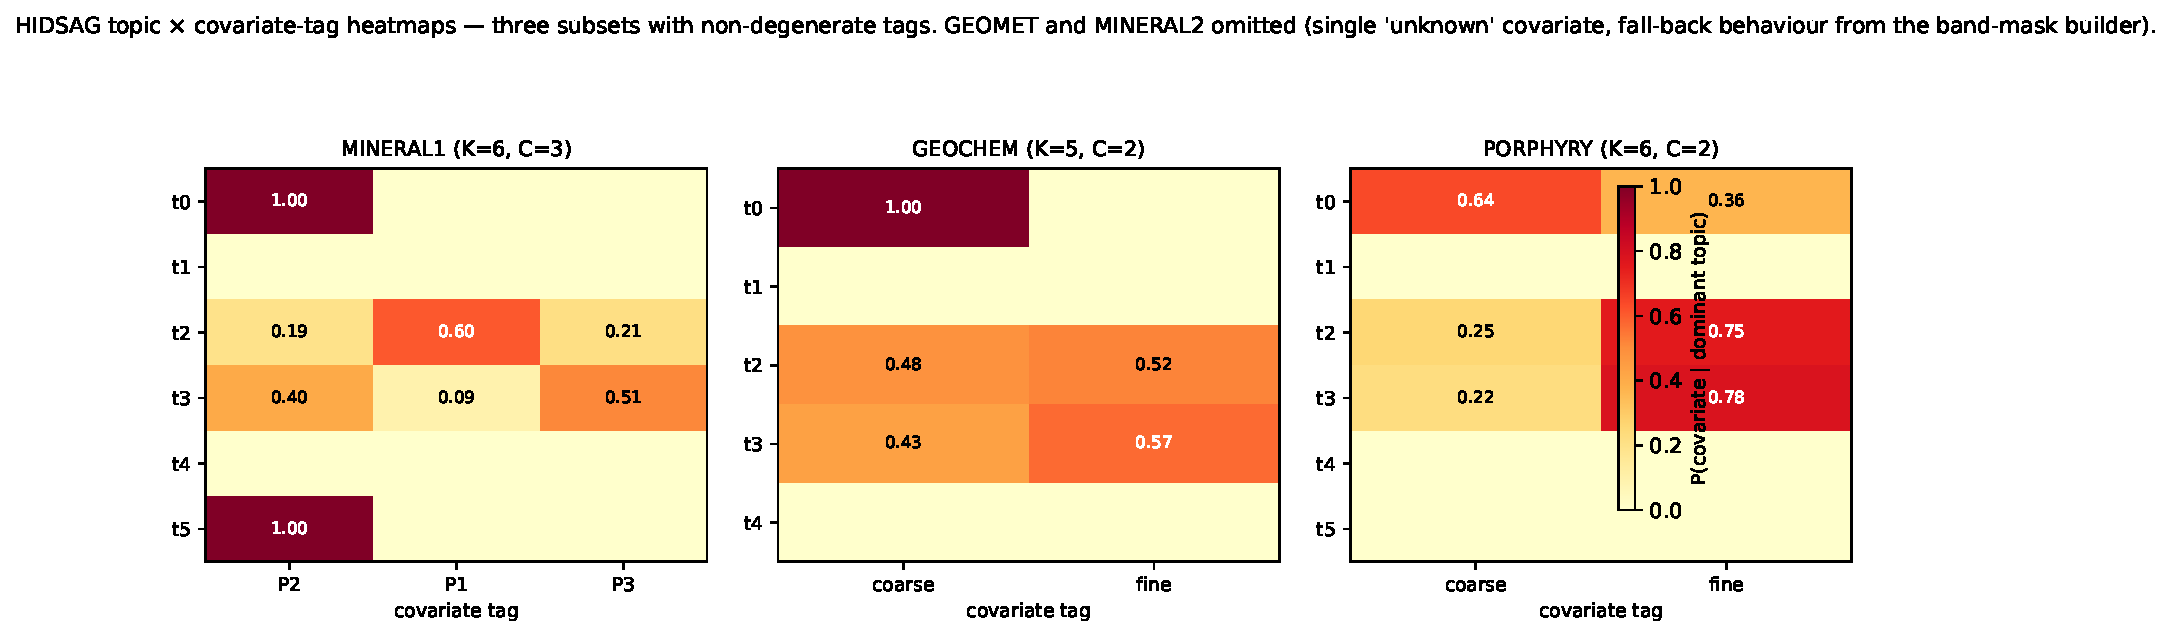
\includegraphics[width=\textwidth]{hidsag-topic-covariate.pdf}
\caption{HIDSAG~\cite{hidsag2023,hidsag2023figshare} topic ×
covariate-tag heatmap on three subsets with non-degenerate
covariates (MINERAL1 with P1/P2/P3; GEOCHEM and PORPHYRY with
coarse/fine). Cell = $P(\text{tag} \mid \text{dominant topic})$.
GEOMET and MINERAL2 are omitted because their available covariates
collapse to a single \texttt{unknown} value at the band-mask
builder's granularity (fall-back behaviour).}
\label{fig:hidsag-cov}
\end{figure}

The continuous mineralogical measurements (Cu rec, Lime cons,
mineral abundances per subset) live in the raw HDF5 source files of
the figshare collection~\cite{hidsag2023figshare} rather than in the
derived JSON exposed by our companion code repository. A future
extension could plug those into the same topic--covariate frame
using ridge plots per topic on the continuous variable, following
the same idiom as Figure~\ref{fig:conf-ridge}.

\section{Why these six figures}

The six figures answer six distinct cognitive questions about the
topic--label relationship:

\begin{enumerate}
\item Heatmap (Fig.~\ref{fig:tc-heatmap}) --- ``which topic--class
cells carry mass?''
\item Per-topic bars (Fig.~\ref{fig:tc-bars}) --- ``what is the
within-topic class distribution shape?''
\item Sankey (Fig.~\ref{fig:tc-sankey}) --- ``where does mass flow
between topic and class?''
\item $\theta$ scatter (Fig.~\ref{fig:theta-scatter}) --- ``do
topics and labels align in the $\theta$-PCA manifold?''
\item Confidence ridge (Fig.~\ref{fig:conf-ridge}) --- ``how sharp
is each topic's posterior?''
\item HIDSAG covariate (Fig.~\ref{fig:hidsag-cov}) --- ``do topics
carry information about the HIDSAG covariate tags?''
\end{enumerate}

Each chosen idiom dominates its question on the cognitive-ergonomic
trade-off between density (information per pixel) and decoding
effort (steps the reader must take to extract a claim). See the
research note in the repository
\texttt{supplementary/journal/research-notes/topic-relational-viz.md}
for the full literature survey that informed the selection.

\bibliographystyle{IEEEtran}
\bibliography{../../bibliography/refs}

\end{document}
